\section{Current System Architecture}

The \textit{SRP} system architecture is fundamentally distributed into two primary segments: 
\begin{itemize}
    \item Company Network;
    \item Client Network.
\end{itemize}

These segments interact and communicate exclusively through a \textit{DMI Console} \cite{service_request_portal}, which acts as a unidirectional bridge, transferring requests from the client network to the internal company network \cite{service_request_portal} \cite{dmi_infrastructure_git}. 

The overall architecture is depicted in the diagram in figure \ref{fig:as-is-system-design} \cite{service_request_portal}.

\begin{figure}[htbp]
  \centering
  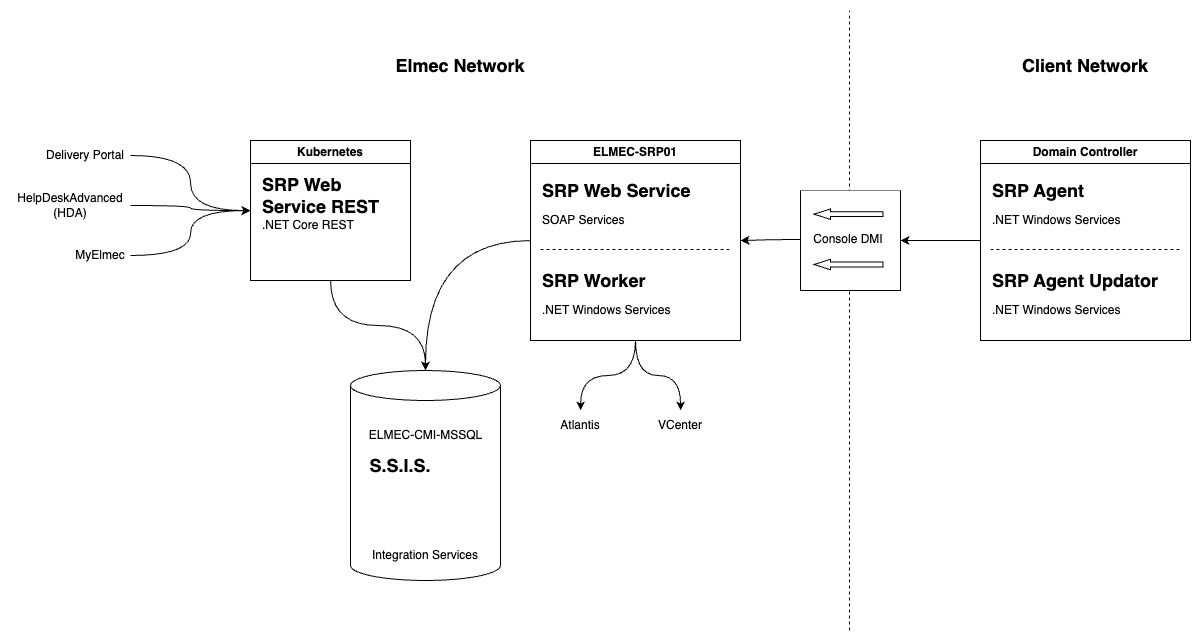
\includegraphics[width=1.0\textwidth]{images/as-is/SRP AS-IS (System Architecture).jpg}
  \caption{AS-IS System Architecture}
  \label{fig:as-is-system-design}
\end{figure}

The system's operational flow involves several key components across both networks, orchestrating the processing of service requests.

\subsection{Main Functionalities and Components}
The current \textit{SRP} system relies on a suite of interconnected components, each serving a specific role in the lifecycle of a service request.

Elmec's Network Components:
\begin{itemize}
    \item \textbf{SRP Web Sevice REST} \cite{srp_webservicerest_git}:  Deployed on a Kubernetes cluster, exposes .NET Core RESTful services \cite{service_request_portal}. It serves as the primary interface for external systems such as:
    \begin{itemize}
        \item \textbf{Delivery Portal}: An internal asset management system used to manage Service Request catalog configuration and Elmec's internal and client servers;
        \item \textbf{HDA (HelpDeskAdvanced)}: An internal ticket management system. Each service request is intrinsically linked to an HDA ticket via an ID, and HDA is responsible for initiating and associating service requests with existing tickets.
        \item \textbf{MyElmec}: A customer-facing portal enabling customers to create, manage, and monitor the various services provided by Elmec (e.g., servers, management software, cloud solutions).
    \end{itemize}
    The \textit{SRP Web Service REST} communicates with the \textit{ELMEC-CMI-MSSQL} server.
    \item \textbf{ELMEC-CMI-MSSQL}: This server hosts the central SQL Server Database for the SRP system. It is the persistent storage layer for all service request data and related information \cite{service_request_portal}.
    \item \textbf{S.S.I.S. (SQL Server Integration Services)}: Running on the \texttt{ELMEC-CMI-MSSQL} server, SSIS packages are crucial for data transformation and import/export operations. They handle the transfer of data, such as master data (e.g., Active Directory users, Organizational Units, AD Groups) sent by SRP Agents, into the database. Each SSIS package is designed to transform the received information for database insertion or vice versa \cite{service_request_portal}.
    \item \textbf{ELMEC-SRP01}: This Windows Server functions as the core engine for service requests within the Elmec network. It houses all the PowerShell scripts associated with individual service requests, which are maintained by the MxS (Managed Services) team \cite{service_request_portal}. Key components residing on \texttt{ELMEC-SRP01} include:
    \begin{itemize}
        \item \textbf{SRP WebServiceSoap}: This component provides SOAP services primarily for communication with the SRP Agent located on the client side. It interacts with the database to retrieve necessary information before exposing it to the agents for Service Request execution \cite{srp_webservice_git}.
        \item \textbf{SRP InternalWorker}: A Windows service that operates similarly to the SRP Agent but executes entirely within the Elmec network. This is utilized for service requests that do not require interaction with the client's network or Active Directory (e.g., managed VM-related service requests). The InternalWorker queries the database every 10 seconds for "internal worker" type jobs (like removing a server from a patching session, or resetting a managed Virtual Machine), connects to the SOAP service, retrieves the Service Request ID and its fields, and initiates job execution. It also monitors logs every 30 seconds to determine the job's status \cite{srp_internalworker_git}.
    \end{itemize}
\end{itemize}

The only component in the client's network is called \textbf{Domain Controller}, which represents the client's Active Directory domain controller, where the communication tools with Elmec are installed. It hosts:
\begin{itemize}
    \item \textbf{SRP Agent (.NET Windows Service)}: Typically, one agent is configured per client domain, specifically for Active Directory (AD) and Exchange-related service requests. This agent performs two main functions \cite{srp_windowsservice_git}:
    \begin{itemize}
        \item Every 8 hours, it reads master data (AD users, OUs, groups) from the domain controller and sends it to \texttt{ELMEC-SRP01} for storage via SSIS.
        \item Every 5 minutes, it queries \texttt{ELMEC-SRP01} for pending Service Requests. Upon finding any, it requests detailed information, loads the corresponding PowerShell script, and executes it. After initiating the script, the agent informs \texttt{ELMEC-SRP01} that the SR is "running" and proceeds to the next SR.
    \end{itemize}
    
    \item \textbf{SRP Agent Updator (.NET Windows Service)}: This service continuously monitors the SRP Agent folder for a file with a \texttt{.new} extension. If detected, it stops the SRP Agent, updates it, and restarts it
\end{itemize}

\subsection{Interactions and Communication between Customers and Company networks}
The Communication between the company network and the customers' networks is a critical aspect of the SRP system's operations and is handled through the \textbf{DMI Console} \cite{service_request_portal}.

The DMI console serves as a key infrastructural component, primarily acting as a communication bridge between the customer's network and Elmec's internal network. Specifically, for the SRP system, the DMI console is responsible for transferring service requests (SR) from the customer's network to Elmec's internal network, although it does not handle traffic in the opposite direction \cite{dmi_infrastructure_git}.

\subsubsection{Operation of the DMI Console}
The connectivity of the DMI appliances to Elmec is established through multiple OpenVPN connections, initiated by the appliance towards the Brunello 4 and Mendrisio Data Centers (for Swiss customers). The DMI consoles are not directly exposed to the Internet and are accessible only by authorized personnel \cite{dmi_infrastructure_git}.

Following recent developments in the DMI, the new consoles use K3S for container management. K3S is a lightweight, certified Kubernetes distribution designed for edge, IoT, and CI/CD environments. It is characterized by being a single binary that reduces external dependencies and uses SQLite as the default database, greatly simplifying installation and management. It already includes essential components such as \textit{containerd} \cite{k3s}.

All consoles are centrally managed via Rancher, and the deployment of the application stack is delegated to ArgoCD, which ensures that container versions are constantly updated. For security reasons, the console in the customer network by default exposes only SSH, while services such as SRP are selectively enabled and only when necessary. All application data present on the consoles is stored on a LUKS (Linux Unified Key Setup) encrypted volume\footnote{A platform-independent hard disk encryption method that can be used to encrypt disks across a wide variety of tools. This not only ensures full compatibility and interoperability between different software but also guarantees that password management occurs in a secure and documented manner \cite{luks}.}, which can only be unlocked if the VPN tunnel is established. The operating system update is performed through a standard Elmec system, called PMD (Patching Management Dashboard) \cite{dmi_infrastructure_git}.